% !TeX spellcheck = en_US

\chapter{Concept}
\label{chap:concept}

This chapter outlines the concept for our smart home chatbot. We begin by exploring the intents defined for the chatbot, which form the foundation of its functionality and aim to surpass the capabilities of current smart home solutions.

The chapter then provides insights gained from preliminary interviews with experts from various domains, including AI technologies, smart home systems, and product development. These interviews provided valuable knowledge, requirements, and ideas that shaped our approach.

Following this, we present a comprehensive set of functional and non-functional requirements for the chatbot, derived from the interview insights and tailored to integrate seamlessly with existing smart home systems, particularly the Bosch Smart Home system.

The chapter proceeds to detail the prototype design and architecture, explaining the rationale behind choosing a client-server model with a customized \gls{llm} at its core. We describe the key components of this architecture and their interactions, providing a clear picture of how the chatbot will function within the smart home ecosystem.

Finally, we discuss the process of collecting example inputs for the chatbot through a survey, which helped us gather a diverse range of natural language queries and commands. This data collection effort ensures that our chatbot can understand and respond to a wide variety of user inputs, enhancing its usability and effectiveness.

\section{Intent Engineering}

Intents are fundamental to the functionality of the chatbot, serving as the core mechanism for understanding and responding to user requests. In the context of our work, an intent represents a specific user goal or action that the chatbot needs to interpret and execute. The careful design and implementation of these intents are crucial for creating a system that can effectively understand and respond to a wide range of user inputs in the smart home domain.

Our approach to intent engineering was systematic and iterative. We began by brainstorming about current smart home systems and voice assistants, focusing on their limitations and potential areas for improvement. This process allowed us to generate a diverse set of ideas for enhancing user interaction with smart home devices.

To organize these ideas and align them with our development strategy, we categorized the proposed intents into three levels of complexity. This categorization was based on the potential implementation challenges and the interdependencies between intents.

For each intent, we developed a structured format consisting of four key elements:
\begin{itemize}
    \item A clear definition of the user's goal
    \item A set of example phrases or queries
    \item Necessary entities or parameters to be extracted
    \item The expected action or response from the system
\end{itemize}

This structured approach ensures consistency across all intents and provides a clear roadmap for implementation.

The decision to define three levels of complexity aligns with our overall iterative approach to prototype development. This strategy allows us to progressively enhance the chatbot's capabilities, starting with basic functionalities and gradually incorporating more advanced features. It also provides natural milestones for testing and evaluation throughout the development process.

In the following subsections, we detail each of these intent categories, showcasing how they collectively contribute to a more flexible and user-friendly smart home interaction experience.

\subsection{Iteration 1: Basic Intents}

\paragraph{Providing Device Status}

\begin{itemize}
    \item \textbf{Intent Name:} GetDeviceStatus
    \item \textbf{Examples:}
    \begin{itemize}
        \item ``What is the temperature in the living room?''
        \item ``What is the status of the thermostat in the living room?''
        \item ``Is it warm in the living room?''
    \end{itemize}
    \item \textbf{Entities:}
    \begin{itemize}
        \item DeviceType (e.g., thermostat, lights)
        \item Room (e.g., living room, bedroom)
    \end{itemize}
    \item \textbf{Action/Response:} Providing information about the specified device in the given room, such as the temperature and power status of a thermostat.
\end{itemize}

This intent aims to provide a more conversational approach to querying device statuses. Unlike existing solutions that require specific device names, our chatbot can understand various formulations, allowing users to ask for the temperature without needing to specify the exact device name or its location.
This intent is especially interesting for the first iteration since the intents of following interations strongly rely on information about the devices of a user. Without data about the devices a user has a smart home chatbot would be quite pointless.

\paragraph{Changing Device Status}

\begin{itemize}
    \item \textbf{Intent Name:} SetDeviceStatus
    \item \textbf{Examples:}
    \begin{itemize}
        \item ``Set the temperature to 22 degrees in the living room.''
        \item ``Turn off the lights in the bedroom.''
        \item ``Make it cooler in the kitchen.''
    \end{itemize}
    \item \textbf{Entities:}
    \begin{itemize}
        \item DeviceType (e.g., thermostat, lights)
        \item Room (e.g., living room, bedroom)
        \item DesiredStatus (e.g., temperature, on/off state)
        \item DesiredValue (e.g., specific temperature, on/off)
    \end{itemize}
    \item \textbf{Action/Response:} Executing the specified action to set the desired status of the mentioned device in the given room, such as adjusting the temperature for a thermostat or turning lights on or off.
\end{itemize}

This intent enhances user experience by allowing natural language commands to control devices. The chatbot interprets a wider range of user commands, enabling users to control their devices more intuitively and without needing to remember specific device names.

\subsection{Iteration 2: Intermediate Intents}

\paragraph{Assistance for Creating Automations}

\begin{itemize}
    \item \textbf{Intent Name:} CreateAutomation
    \item \textbf{Examples:}
    \begin{itemize}
        \item ``Set up an automation for turning off lights at 10 PM.''
        \item ``Create a rule to adjust thermostat settings when I leave home.''
        \item ``Can you help me with automating my smart blinds?''
        \item ``Notify me if any windows are open.''
    \end{itemize}
    \item \textbf{Entities:}
    \begin{itemize}
        \item DeviceType (e.g., lights, thermostat, blinds)
        \item TriggerEvent (e.g., time-based, occupancy, temperature change)
        \item Condition (optional, e.g., specific temperature threshold)
        \item Action (e.g., turn off, adjust settings)
        \item Location (optional, e.g., living room, bedroom)
    \end{itemize}
    \item \textbf{Action/Response:} Assisting the user in defining and setting up a smart home automation, including specifying the devices involved, the triggering event, any conditions, and the desired actions. The chatbot may also provide suggestions for common automation scenarios.
\end{itemize}

Creating automations is a common use case in smart home systems. This intent aims to streamline the process, allowing users to set up complex automations through simple conversational interactions, thus reducing the need for technical knowledge or precise phrasing.

\paragraph{Interpret the Device Control}

\begin{itemize}
    \item \textbf{Intent Name:} DeviceControlInterpretation
    \item \textbf{Examples:}
    \begin{itemize}
        \item ``Why did the lights in the bathroom turn on just now?''
        \item ``Can you explain the reason for the thermostat adjusting the temperature?''
        \item ``What triggered the blinds to open in the living room?''
    \end{itemize}
    \item \textbf{Entities:}
    \begin{itemize}
        \item DeviceType (e.g., lights, thermostat, blinds)
        \item Location (optional, e.g., bathroom, living room)
        \item Action (e.g., turn on, adjust temperature, open)
        \item TriggerSource (e.g., automation, manual activation)
        \item Timestamp (optional, for specifying a time reference)
        \item Reason (optional, e.g., reason for an automation that the user provided when creating it)
    \end{itemize}
    \item \textbf{Action/Response:} Providing an explanation for recent smart home device actions. The chatbot interprets the cause of device events, distinguishing between automation-driven events and those triggered manually by the user. It may also consider time-based context when explaining device actions.
\end{itemize}

This intent addresses a gap in current systems by explaining the reasons behind device actions. It improves transparency and user trust in smart home systems by providing clear explanations for automated and manual device actions.

\subsection{Iteration 3: Complex Intents}

\paragraph{Analyzing Energy Consumption}

\begin{itemize}
    \item \textbf{Intent Name:} AnalyzeEnergyConsumption
    \item \textbf{Examples:}
    \begin{itemize}
        \item ``Can you analyze the energy consumption in my home?''
        \item ``Provide insights into power usage over the last week.''
        \item ``How can I optimize energy consumption in the living room?''
    \end{itemize}
    \item \textbf{Entities:}
    \begin{itemize}
        \item AnalysisType (e.g., overall consumption, specific devices)
        \item TimeFrame (e.g., last week, last month)
        \item Room (e.g., living room, kitchen)
    \end{itemize}
    \item \textbf{Action/Response:} Generating a detailed analysis of energy consumption based on the specified parameters. It includes insights into overall energy usage, specific device contributions, and recommendations for optimizing energy consumption in the specified room or timeframe.
\end{itemize}

Energy consumption analysis is a valuable addition to smart home capabilities. This intent provides users with actionable insights into their energy use, helping them to make informed decisions about energy efficiency and cost savings.


%% Auslagern in eigenes chapter??? %%
\section{Preleminary Interviews to Gain Knowledge, Requirements and Ideas}
Preceding to further actions Interviews with a few individuals were conducted to gain knowledge, requirements and ideas for this thesis.
All of the four interviewed were from different domains: One is a researcher and has knowledge in \gls{ai} technologies or more precisely about \glspl{llm} while the three other interviewees are from Bosch.
One of them is working in \qq{AskBosch} but also has expertise in the Smart Home and \gls{iot}. 
The other two are both from Bosch Smart Home where one is a Software Developer and the other a Product Developer.
Therefore a diverse group of interviewees has been formed.

The interview was designed to be open but some guided questions were formulated which were selected based on the domain of the interviewed since not all questions met every present domain.
For example it would have not make sense to ask a Smart Home Software Developer about recent tools or the architecture of \gls{llm}-based applications.
In the following all guided questions are listed:

\begin{enumerate}
    \item \textbf{Feasibility and Key Considerations} \\
    What are your thoughts on the feasibility of a smart home chatbot for providing explainability and enhancing user experience?
    \item \textbf{Interesting Intents}
    From your perspective, what could be interesting intents for a smart home chatbot to address complex user queries?    
    \item \textbf{Selected Intents}
    What is your opinion on the specific intents that have been selected for the chatbot development?    
    \item \textbf{Tools/Technologies/Models}
    In your research experience, what tools, technologies, or models would you recommend for developing a chatbot tailored for smart home applications?
    Would you chose a large language model and input context and user request into it or rather a NLP pipeline that chooses further actions based on the user request?   
    \item \textbf{Data Organization}
    How would you suggest organizing and feeding data to the chatbot, considering the complexity of smart home scenarios?    
    \item \textbf{Common Issues/Pitfalls}
    Based on your expertise, what are the common issues or pitfalls researchers may encounter when developing chatbots for specialized domains like smart homes?
    \item \textbf{Evaluation of Success}
    How would you propose evaluating the success of a smart home chatbot, especially in terms of providing explainability and user-centric interaction? 
    \item \textbf{Data Sources for the Chatbot}
    Can you identify potential sources from which data for the chatbot could be extracted to address user queries about the smart home?
    \item \textbf{Accessibility of Data}
    Do you foresee any challenges or limitations in accessing the identified data sources for the chatbot development?
           
\end{enumerate}

\subsection{Interview Summary}
\label{sec:interview_summary}

The following summary captures the insights and recommendations from these interviews.

\subsubsection{Feasibility and Key Considerations}

The feasibility of implementing a smart home chatbot was generally supported by all interviewees, albeit with some caveats:

\begin{itemize}
    \item \textbf{Technical Feasibility}: It is crucial to use proven frameworks and consider whether an \gls{llm} is necessary or if Named Entity Recognition (NER) would suffice, particularly given budget constraints. \glspl{llm} require significant resources, which may be impractical without a robust client-server architecture.
    \item \textbf{User Experience}: The chatbot must simplify user interactions with smart home devices, removing the need for exact device names and understanding user patterns for better automation.
    \item \textbf{Market Viability}: There are concerns about privacy and trust, which affect the acceptance of AI and chatbots in the market.
\end{itemize}

\subsubsection{Interesting and Selected Intents}

The interviewees proposed several useful intents for the chatbot:

\begin{itemize}
    \item \textbf{Device Control}: Activating or deactivating devices, querying the status of doors and windows, and setting temperatures.
    \item \textbf{Automation Assistance}: Simplifying the creation of automations, such as scheduling device operations and explaining device actions.
    \item \textbf{Energy Management}: Providing insights into energy consumption and optimization suggestions.
    \item \textbf{User-Specific Recommendations}: Customizing suggestions based on user behavior and preferences, such as recommending automations for commonly adjusted settings.
\end{itemize}

\subsubsection{Tools, Technologies, and Models}

Several tools and technologies were recommended for developing the chatbot:

\begin{itemize}
    \item \textbf{LLM vs. NER}: While \glspl{llm} offer broad capabilities, \gls{ner} may be sufficient for specific use cases. But a \gls{llm} fine-tuned or customized to suit a specific application can also work out great.
    \item \textbf{Frameworks and Platforms}:  Tools like Microsoft Bot Framework\footnote{\url{https://github.com/microsoft/botframework-sdk}}, Conversational Language Understanding\footnote{\url{https://learn.microsoft.com/en-us/azure/ai-services/language-service/conversational-language-understanding/overview}}, Dialogflow\footnote{\url{https://cloud.google.com/dialogflow}}, and LangChain\footnote{\url{https://www.langchain.com/}} were mentioned as tools for different use cases. Except Dialogflow and the Azure Service Conversational Language Understanding they are open source. Potentially a Spring Boot\footnote{\url{https://spring.io/}} or Node.js\footnote{\url{https://nodejs.org/}} application could suit the use case of this thesis.
    \item \textbf{Data Management}: Organizing data with configurations that map intents to actions, and ensuring the chatbot can correctly interpret inputs is vital.
\end{itemize}

\subsubsection{Data Organization and Sources}

Effective data organization and source identification are a key aspect for achieving the desired chatbot functionality:

\begin{itemize}
    \item \textbf{Configurations and Scenarios}: Initial iterations should use predefined configurations, mapping intents to device actions.
    \item \textbf{Data Collection}: Gathering diverse user inputs to train models and create accurate annotations is essential for generalizability. They are also useful for the evaluation of the performance of the chatbot
    \item \textbf{Potential Sources}: Logs from smart home devices , external services, and user behavior data should be considered. For the beginning the most important data is about the devices of a user since it is crucial for all of the defined intents and the most essential part of a smart home.
\end{itemize}

\subsubsection{Common Issues and Pitfalls}

While the initial intention was to find out about general issues and pitfalls that often occur in the development of chatbot-powered applications in the interviews the direction 
Several potential challenges were highlighted:

\begin{itemize}
    \item \textbf{Complexity of Automations}: Creating sophisticated automations might be challenging and require a balance between simplicity and functionality.
    \item \textbf{Data Privacy and Trust}: Addressing user concerns about privacy and the reliability of AI-generated information is crucial.
    \item \textbf{Resource Constraints}: Ensuring sufficient computational resources for \glspl{llm}, if used, and managing the cost of development.
\end{itemize}

\subsubsection{Evaluation of Success}

The success of the smart home chatbot can be evaluated through:

\begin{itemize}
    \item \textbf{Performance Metrics}: Comparing expected outcomes with actual results using metrics like the F1 score.
    \item \textbf{User Experience}: Conducting user evaluations to assess satisfaction and the effectiveness of interactions.
    \item \textbf{Prototyping and Testing}: Iterative testing with real users to refine the chatbot's capabilities and ensure it meets user needs.
\end{itemize}

\subsection{Conclusion}

The interviews provided a comprehensive understanding of the requirements and considerations for developing a smart home system chatbot. Key insights include the importance of choosing the right technologies, ensuring robust data management, and addressing user privacy concerns. By focusing on practical intents and leveraging existing frameworks, the development of a user-friendly and effective smart home chatbot is achievable.


\section{Requirements of the Chatbot}

This section outlines the functional and non-functional requirements of the chatbot designed for integration with smart home systems, particularly focusing on the Bosch Smart Home system.
They are formulated in a general way and not from the view of a specific role.
The requirements were gathered primarily by drawing conclusions from the preliminary interviews.

To shortly discuss requirement types it is well known that  software requirements can be classified into two categories: \glspl{fr} and \glspl{nfr}. 
A common ground is that \glspl{fr} describe what the system shall do (describe specific behaviors and capabilities of the system) where in contrast \glspl{nfr} describe how a system shall do something (focus on quality attributes, constraints, and overall system characteristics).
But in practice, researchers unveiled that it is hard to draw a line between these two types of requirements. \glspl{nfr} often stay very vague and are therefore hard to analyze \cite{nfr_fr}.
But because it is still the most widespread definitions, it is applied in this work.

The following requirements provide a comprehensive foundation for developing a smart home chatbot that is functional, secure, and user-friendly. The focus on integrability with existing systems, particularly the Bosch Smart Home system, ensures practical applicability, while attention to maintainability and cost-effectiveness supports sustainable deployment.

\subsection{Functional Requirements}

\begin{itemize}
    \item \textbf{Intent Addressing}: The chatbot should accurately address the defined intents. The extent of this capability depends on the progress made by the deadline of this thesis.
    
    \item \textbf{Language Support}: The chatbot should support both German and English languages. It should respond in the same language as the user's input. For example, if a user query is in German, the chatbot should reply in German, and likewise for English.
    
    \item \textbf{Integrability}: The chatbot should be easily integrable into existing smart home systems, particularly the Bosch Smart Home system. Integration should require only a mapper class/code capable of splitting the chatbot's output into the natural language response for the user and a system output (a \gls{json} in this work) that maps to the smart home system's functionalities.
    
    \item \textbf{Context Awareness}: The chatbot should maintain context within a session to handle follow-up questions and commands effectively, providing a more natural interaction experience.
    
    \item \textbf{Command Execution}: The chatbot should be capable of executing specific commands related to smart home functionalities, such as turning devices on or off, adjusting settings, and providing status updates.
    
    \item \textbf{Error Handling}: The chatbot should be able to handle errors gracefully, providing helpful feedback to users when it cannot understand a request or when an action cannot be completed.
\end{itemize}

\subsection{Non-Functional Requirements}

\begin{itemize}
    \item \textbf{Security and Safety}: The chatbot may handle sensitive data, including information about users' devices and smart home system logs. It is crucial to ensure this information is not exposed to unauthorized parties. Self-hosting the \gls{llm} could enhance security.
    
    \item \textbf{Cost-Effectiveness}: The solution should be cost-effective since \gls{llm}-based software can get expensive easily. Self-hosting the \gls{llm} could reduce costs associated with third-party services.
    
    \item \textbf{Usability}: The chatbot should be user-friendly, providing clear and concise responses. The interface should be intuitive for users with varying levels of technical expertise. 
    
    \item \textbf{Performance}: While performance is not the primary focus for this proof of concept, the chatbot should respond within a reasonable time to avoid negatively impacting usability. Quick response times are essential for maintaining a smooth user experience.
        
    \item \textbf{Maintainability}: The chatbot system should be easy to maintain and update. Clear documentation and modular design can facilitate easier maintenance and the addition of new features which is always nice to have but also necessary for the Iterative approach of this thesis.
\end{itemize}

\section{Protoype Design and Architecture}
\label{sec:design}
In this section, we outline the design and architecture of the smart home chatbot prototype. This prototype aims to facilitate seamless and intuitive interactions between users and their smart home devices by leveraging advanced natural language processing (NLP) techniques and smart home integration capabilities.

\subsection{Overview}
Two primary design options were available for this thesis: creating a \gls{nlp} pipeline with \gls{ner} to detect intents and trigger actions, or leveraging a \gls{llm} for the entire process. After careful consideration, the \gls{llm} approach was deemed more suitable for the designed intents due to its potential to significantly reduce manual effort.

The \gls{llm} approach simplifies the process by requiring only the customization or fine-tuning of the model, necessitating the provision of an appropriate prompt and the relevant data for the prompt. This is particularly advantageous for intents that involve complex analyses, such as determining the reasons behind higher energy consumption in the current month compared to the previous one. Using a \gls{llm} eliminates the need to develop intricate deterministic functions to achieve such complex tasks. In essence, a \gls{llm} can handle a broader range of messages and data formats without the necessity of meticulously defining each scenario.

For the base architecture of the application using the aforementioned approach, three main options were considered:
\begin{enumerate}
    \item \textbf{Using an API from an \gls{llm} provider like OpenAI}: This option provides access to powerful, state-of-the-art models without the need for extensive infrastructure. However, it involves recurring costs and reliance on third-party services.
    \item \textbf{Self-hosting an \gls{llm}}: This approach offers more control over the model and data, potentially enhancing privacy and customization. Nonetheless, it requires significant resources for infrastructure and maintenance.
    \item \textbf{Integrating the \gls{llm} directly into the corresponding Smart Home App}: This would allow for seamless integration and potentially faster response times. However, the constraints of mobile devices, such as limited processing power and storage, could pose significant challenges. A tiny model would probably be needed to use.
\end{enumerate}

After evaluating these options, a client-server architecture was chosen as the most suitable approach. This architecture involves hosting the \gls{llm} on a server and having the client application communicate with the server to access the \gls{llm}'s capabilities. The client-server model offers several advantages:

\begin{itemize}
    \item \textbf{Cost Reduction}: If a free server is available or an underutilized server can be used, this approach can significantly reduce operational costs compared to continuously using a third-party API.
    \item \textbf{Scalability and Flexibility}: The server can be scaled up or down based on the application's needs, providing flexibility in handling varying workloads.
    \item \textbf{Enhanced Control and Customization}: Self-hosting the \gls{llm} allows for greater control over the model, enabling customizations tailored to specific application requirements and user needs.
    \item \textbf{Improved Data Privacy and Security}: By managing the \gls{llm} on a private server, the risks associated with transmitting sensitive data to external providers are minimized.
\end{itemize}

Overall, the client-server architecture was selected to balance the benefits of leveraging advanced \gls{llm} capabilities while maintaining cost-efficiency, scalability, and enhanced control over the application's functionality and data management. This architecture serves as the foundation for implementing the smart home application's intelligent features, ensuring robust and efficient operation.

The client-server architecture, depicted in Figure \ref{fig:client-server-architecture}, illustrates the fundamental components and their interactions. The server hosts a customized \gls{llm} that handles the complex natural language processing tasks. The client side, which is part of the smart home application, includes the Chat UI, Chat History, and Smart Home Data. 
The Chat UI enables and is essential for user interaction, while the Chat History maintains a record of the conversation that is also shown in the UI of course. 
The Smart Home Data component integrates with various smart home devices to provide the necessary context and information for the \gls{llm}.

\begin{figure}[h]
    \centering
    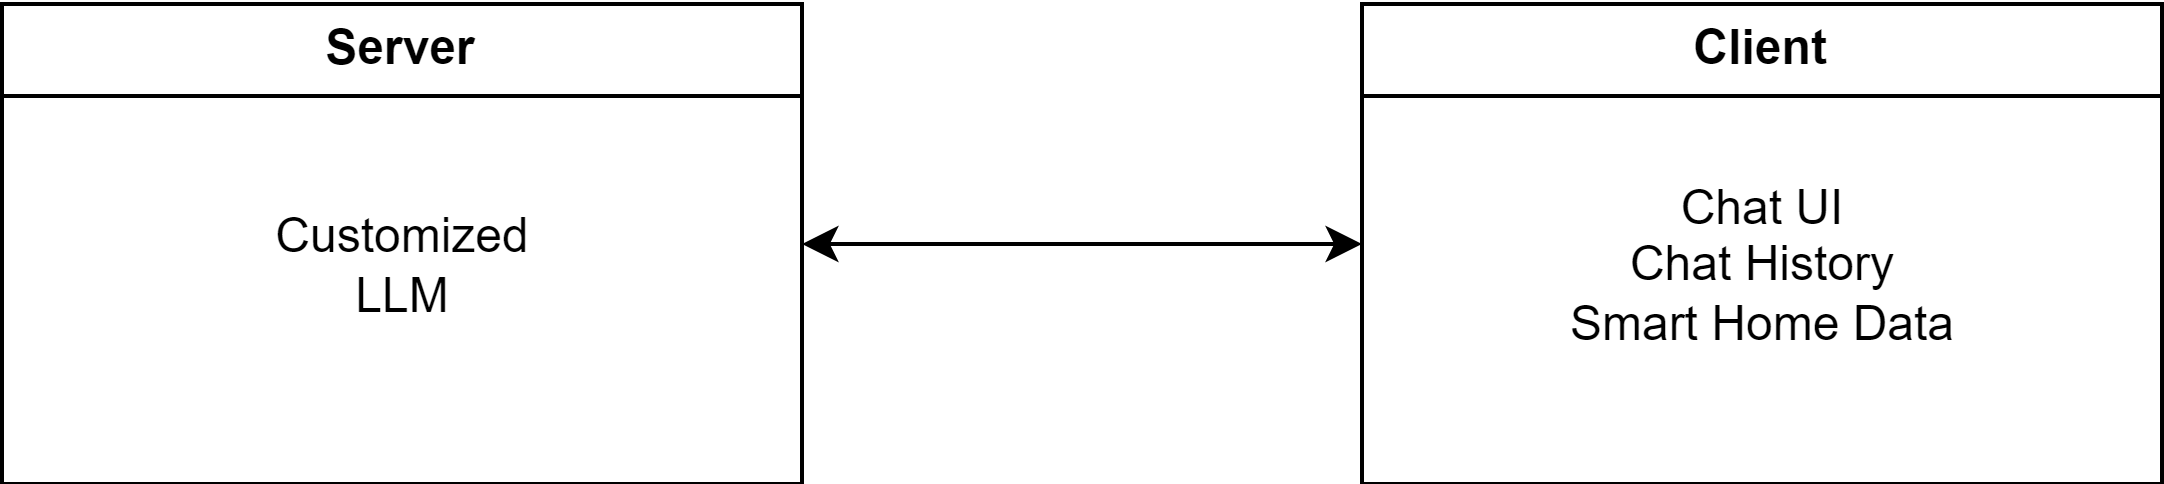
\includegraphics[width=0.98\textwidth]{graphics/ClientServer.png}
    \caption{Client-Server Model of the Chatbot Application}
    \label{fig:client-server-architecture}
    \end{figure}


\subsection{System Architecture}

The chatbot application implements an architecture inspired by the Model-View-Controller (MVC) pattern, adapted for Android development and aligned with the conceptual architecture diagram.
It can be seen in \cref{fig:architecture}.

The Model is represented by the Data Manager, which encapsulates the business logic and data operations related to smart home devices. It interfaces with the Smart Home System to manage device states and communications.

The View component is primarily implemented in the UI module, handling the user interface and interaction elements, including the chat message display and input field. The Message Adapter facilitates efficient rendering of chat messages.

The Controller role is distributed across multiple components. The API Client and Request Builder acts as a primary controller, mediating between the UI and the Data Manager. It processes user inputs, constructs API requests, and manages communication with the Customized \gls{llm} server. The Response Handler processes server responses, updating the UI and Data Manager as needed.

This architecture incorporates modern Android development practices, such as asynchronous operations for API calls and efficient list rendering, enhancing performance and user experience while maintaining a clear separation of concerns aligned with the MVC pattern.


\begin{figure}[h]
\centering
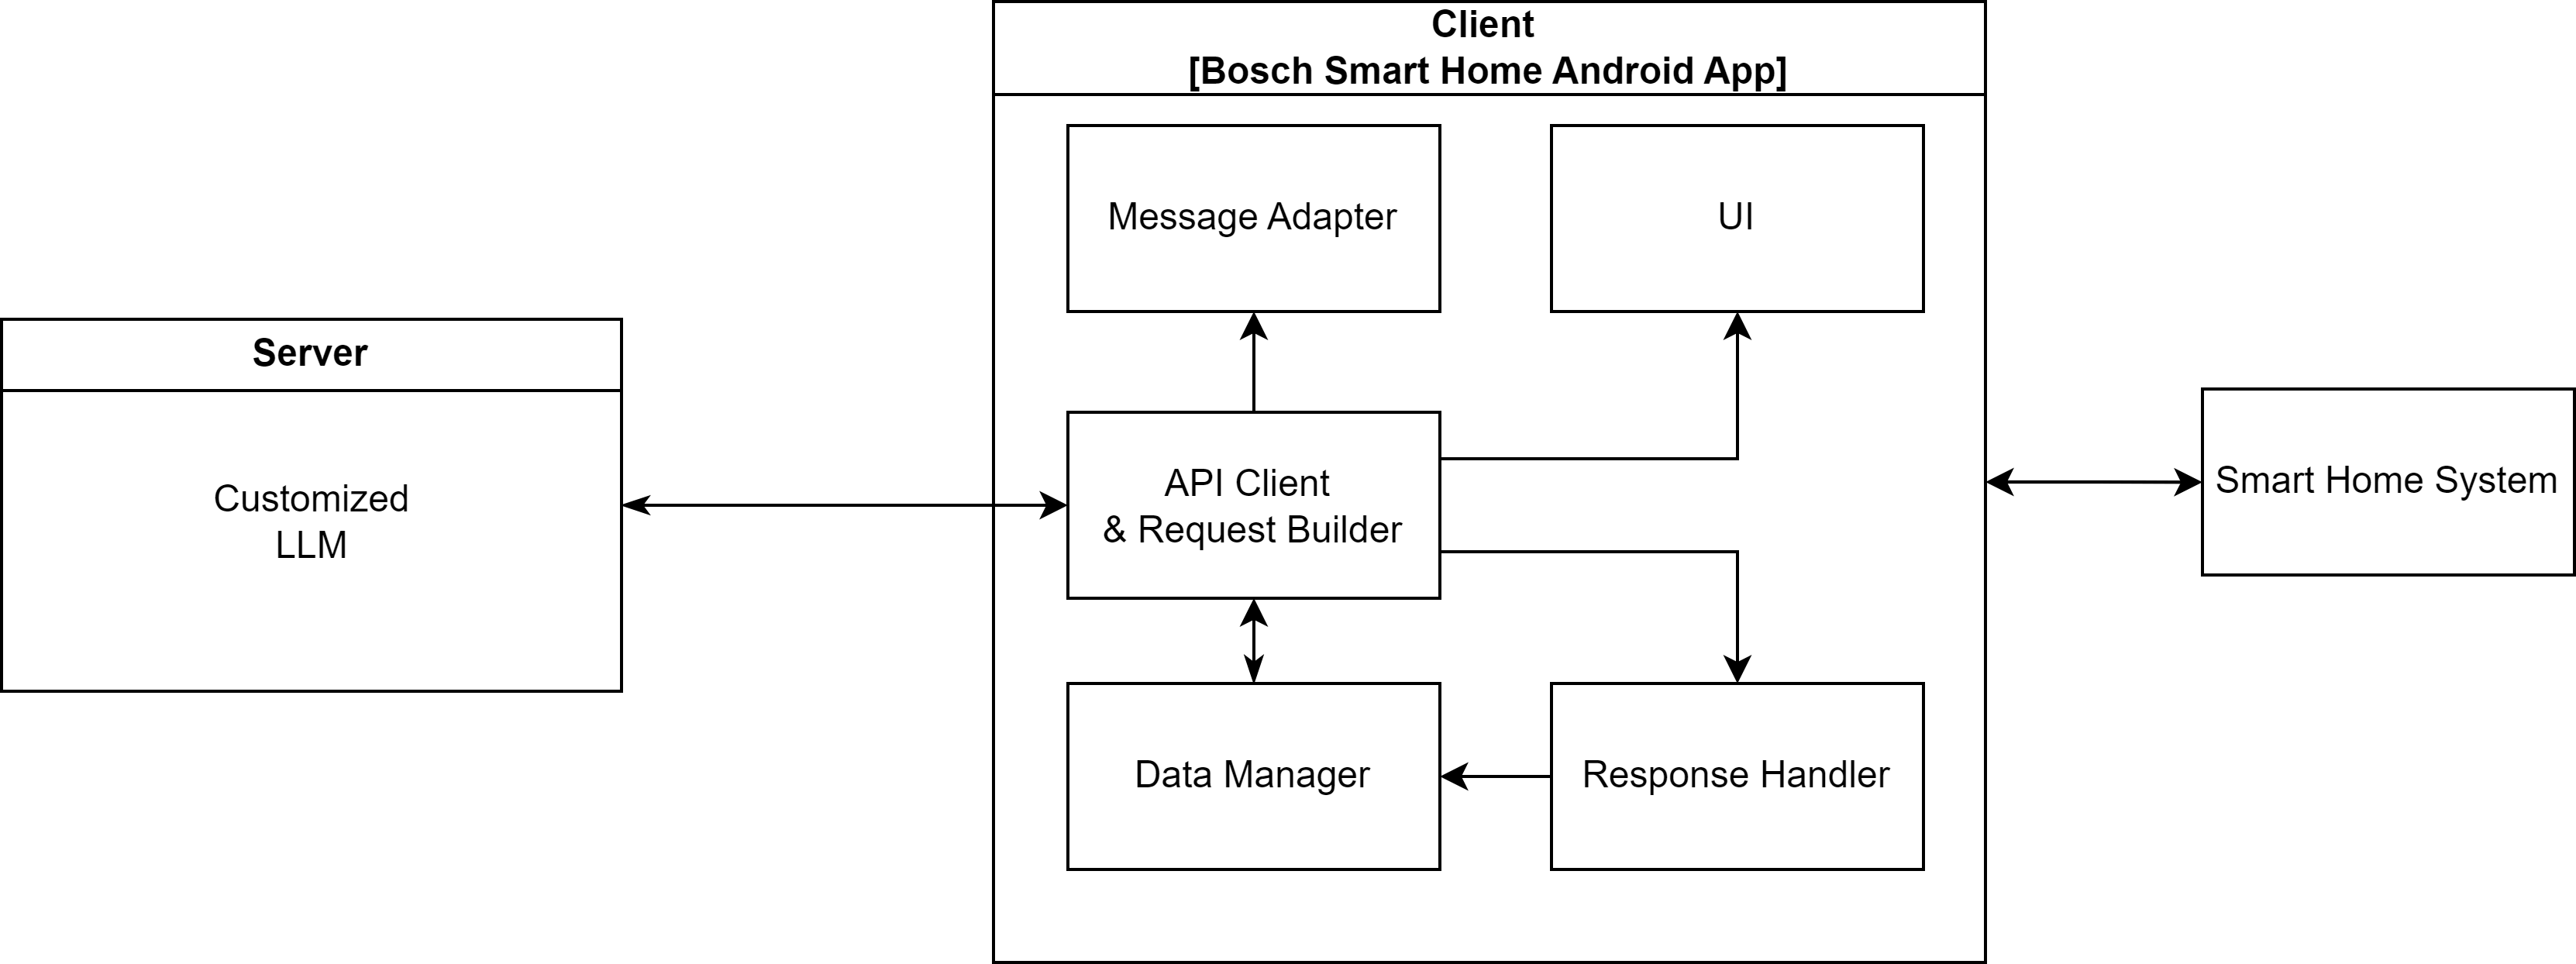
\includegraphics[width=0.98\textwidth]{graphics/ConceptOverview.png}
\caption{High-Level Architecture of the Smart Home Chatbot Prototype}
\label{fig:architecture}
\end{figure}

\subsubsection{UI Module}
The UI module serves as the primary interface between the user and the smart home chatbot system.
The UI module is designed to be intuitive and responsive, providing real-time updates as users interact with the system or as device states change.
It displays each token of the \gls{llm} when received and therefore creates the impression that it is writing with the user.

\subsubsection{Message Adapter}
\label{subsec:messageadapter}
The Message Adapter is responsible for efficiently managing and displaying chat messages within the UI. Its primary functions include:
\begin{itemize}
    \item Message Rendering: Converts message data into viewable UI elements.
    \item Chat History Management: Handles loading, storing, and displaying conversation history.
    \item Message Differentiation: Visually distinguishes between user messages and assistant messages
    \item Dynamic Updates: Allows for real-time addition and modification of messages without requiring a full UI refresh.
\end{itemize}
This module enhances the user experience by ensuring smooth scrolling and efficient memory usage, even with long conversations.

\subsubsection{API Client \& Request Builder}
\label{subsec:apiclient}
The API Client \& Request Builder module serves as the communication bridge between the client application and the server-side \gls{llm}. Its key responsibilities include:
\begin{itemize}
    \item Request Formation: Constructs properly formatted API requests based on user inputs and system state.
    \item Communication Protocol Management: Handles HTTP/HTTPS requests, including authentication and error handling.
    \item Response Parsing: Performs initial parsing of server responses for further processing.
    \item Asynchronous Operations: Manages non-blocking API calls to ensure a responsive user interface.
\end{itemize}
This module is crucial for maintaining efficient and reliable communication with the server-side components of the system.

\subsubsection{Data Manager}
The Data Manager module acts as the central data handler for the client-side application. Its primary functions encompass:
\begin{itemize}
    \item Device State Management: Maintains an up-to-date record of all connected smart home devices and their current states.
    \item Chat History Persistence: Maintains a chat history of user and chatbot messages.
    \item Data Retrieval: Provides methods for other modules to access relevant data efficiently.
    \item Smart Home System Interface: Manages communication with the Smart Home System for device control and state updates.
\end{itemize}
This module ensures data consistency across the application and provides a unified interface for data-related operations.

\subsubsection{Response Handler}
\label{subsec:responsehandler}
The Response Handler module processes the responses received from the server and orchestrates appropriate actions within the client application. Its key responsibilities include:
\begin{itemize}
    \item Response Interpretation and Splitting: Analyzes the server's response to determine required actions. For this the response needs to splitted into a natural language answer and a format that can be transformed into system actions.
    \item Action Execution: Triggers appropriate functions in other modules based on the interpreted response.
    \item UI Update Coordination: Ensures the user interface reflects the latest system state and server responses.
    \item Error Handling: Manages and communicates any errors or unexpected responses from the server which in the end should be displayed by the UI.
\end{itemize}
This module plays a critical role in translating server responses into meaningful actions and feedback within the client application.

\subsection{Supported Devices}
\label{subsec:devices}
To keep the complexity of the system low only a few devices were selected to be supported to be handled by the chatbot.
The selected devices are thermostat, door-window contact and smart plug which all are of the first generation of Bosch devices since we had them easily available in the office.
The devices match the initial idea of the chatbot to help in the enregy crisis and global warming through analyzing capabilites of a users' smart home.
The main complexity is generated by the need to filter out relevant information from the real-time-state of each device and especially by the device controlling intent, because the product palette of Bosch is broadly diversified with different functions needed for controlling each device. 
This selection of devices also makes testing and evaluation of the chatbot easier and serves as a consistent setup throughout the thesis.

\section{Collection of Example Inputs for a Smart Home Chatbot}
\label{sec:collectinputs}
To gather a diverse set of example inputs for our smart home chatbot, we conducted a survey using Microsoft Forms\footnote{\url{https://forms.office.com/}}. The survey was designed to collect typical user queries and commands in both German and English. A total of 13 participants contributed to the study, including 6 from Bosch Smart Home and 7 external participants (primarily university students, with some others). The age distribution of the participants varied, with the majority being under 30 years old.

The survey presented participants with a scenario where they owned smart devices as mentioned in \cref{subsec:devices}. They were asked to formulate queries and commands for various situations related to these devices. The questionnaire included the following situations for which the participants should formulate prompts to a smart home chatbot:

\begin{enumerate}
    \item Check if one or more devices are turned on or off.
    \item Inquire about the temperature of one or more thermostats.
    \item Change the status of your favorite device (temperature, on/off).
    \item Create an automation to save electricity or heating costs.
    \item Investigate why a device has just been turned on unexpectedly.
    \item Inquire about increased energy consumption for the current month.
    \item Analyze if there are specific times when your smart home consumes more energy than at other times and what could be the reason for this (e.g., an automation or different electricity prices at different times). How would you ask the chatbot to help you with this analysis?
    \item The month before last, your energy costs were higher than last month. You suspect this might be related to weather conditions (temperature, less power generation from your own solar panels) or other external circumstances. However, you don't rule out the possibility that you simply consumed more electricity. How would you ask the chatbot to assist you with this analysis?
\end{enumerate}

Participants were encouraged to be creative in their responses, using room names or inventing device names as needed. They were also given the option to provide multiple formulations for each situation by filling out the questionnaire multiple times.

This approach allowed us to collect a wide range of natural language inputs, reflecting various user preferences and linguistic styles and specifically matching the Intents we defined for out chatbot. The gathered data serves as a foundation for improving the chatbot's natural language understanding capabilities, ensuring it can handle diverse user queries effectively.
Additionally we used a big part of it for evaluating the output quality of the chatbot using different language models.
%\section{further parts of the prototype - NLP Pipeline, Integration into the Bosch SH App,...}

%\blinddocument
